\chapter{Project Architecture}\label{ch:B}

\section{Hierarchy of users}
Each structure has its own hierarchy. And this is also present in our project. We would like to show you our hierarchy. (See Figure \ref{fig:Hierarchy}).

\begin{figure}[h!]
    \centering
    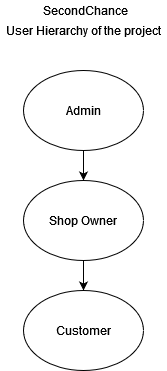
\includegraphics[scale=0.6]{figures/Hierarchy.png}
    \caption{User types}
    \label{fig:Hierarchy}
\end{figure}

\section{User case diagram}
Through the user case diagram, you can understand how our web-site works. Here is a user case diagram.(See Figure \ref{fig:user-case}).
In our case, there are three roles - Admin, Shop Owner, Customer.  Each of them has their own individual roles that are interconnected.  The admin can add or remove shop owners and stores.  And in turn, Shop Owners create or delete a store product, and they can also edit products.  For example, they can change the time of the auction.
Customers can purchase items only after registration.

\begin{figure}[h!]
    \centering
    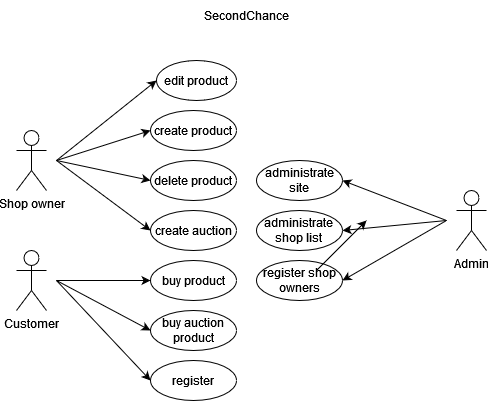
\includegraphics[scale=0.6]{figures/user-case.png}
    \caption{User-case diagram}
    \label{fig:user-case}
\end{figure}
\clearpage


\section{Activity diagram}
The activity diagram describes the actions that are performed on the web-site. Clients should have a registered account to purchase the product. If the client does not have it, he would not be able to buy selected products. Next step is checking if the product is still available or not. If not, the actions will end. When a selected product is available, the next action is payment. Only on condition that the payment goes through, the order is confirmed. If payment does not go through, the process ends without purchasing the product. (See Figure \ref{fig:activity-shop}).

\begin{figure}[h!]
    \centering
    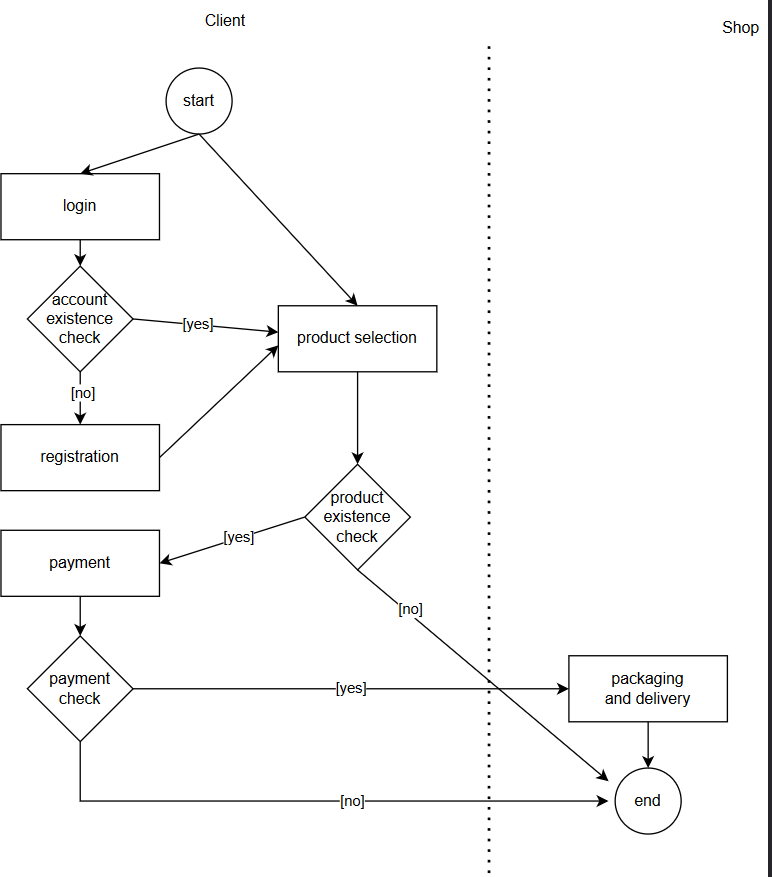
\includegraphics[scale=0.92]{figures/activity-shop.jpg}
    \caption{Activity-shop diagram}
    \label{fig:activity-shop}
\end{figure}
\clearpage

The last diagram was about the shop-system. This one shows the functionality of the auction system. (See Figure \ref{fig:activity-auction}).

\begin{figure}[h!]
    \centering
    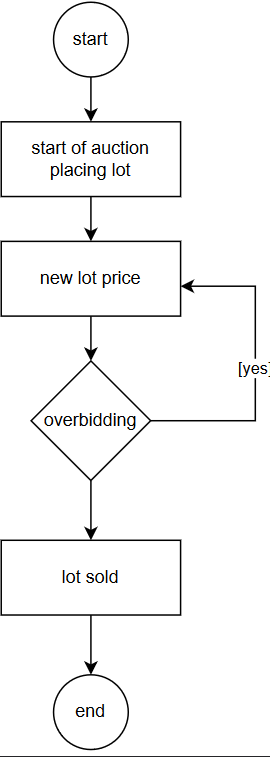
\includegraphics[scale=0.6]{figures/activity-auction.png}
    \caption{Activity-auction diagram}
    \label{fig:activity-auction}
\end{figure}

